%________________________________________________________________________________________________
\documentclass{beamer}
%________________________________________________________________________________________________
\usepackage[french]{babel} 
\usepackage[utf8]{inputenc} 
\usepackage[T1]{fontenc} 
\usepackage{graphicx}
\usepackage[utf8]{inputenc}
\usepackage{fancyhdr}
\usepackage{geometry}
\usepackage{tabularx,tabulary}
\usepackage{movie15}
%________________________________________________________________________________________________
\title{3I013 Soutenance 6 Mai 2019}
\author{Nicolas CASTANET\\Maël FRANCESCHETTI\\Daoud KADOCH\\Fabien MANSON\\}
%________________________________________________________________________________________________
%ce theme est le plus clean de Beamer le truc a ne pas utiliser c'est 'Warsaw'
\usetheme{default}
%suppression de la barre de navigation inutile
\setbeamertemplate{navigation symbols}{}
\setbeamertemplate{frametitle}[default][center]

%\logo{
\includegraphics[height=0.5cm]{logo_sorbonne.png}}

%________________________________________________________________________________________________
\addtobeamertemplate{footline}{
	\begin{flushright}
	\vbox{\insertframenumber/\inserttotalframenumber}
	\end{flushright}}

%________________________________________________________________________________________________
\begin{document}


	\begin{frame}
		\begin{center}
		\date{}
		\maketitle
		\end{center}
	\end{frame}
	
%________________________________________________________________________________________________	
	
	\begin{frame}
		\section{}
		\begin{center}
		\frametitle{Sommaire}
		\tableofcontents{}
		\end{center}
	\end{frame}
	
	%________________________________________________________________________________________________
	
	\begin{frame}
		\section{La Demande du Client}
		\begin{center}
		\frametitle{La Demande du Client}
		\begin{itemize}
		    \item Le client souhaite effectuer des rondes avec un drone Bebop 2\\
		    \item Le drone doit voler de manière autonome en suivant un plan de vol prédéfini \\
		    \item Le retour vidéo du drone doit être redirigé à un iPod touch qui sera placé dans un masque FPV pour permettre à l'utilisateur de voir comme s'il était à la place du drone\\
		\end{itemize}
		   
		\end{center}
	\end{frame}
%________________________________________________________________________________________________	
	\begin{frame}
		\section{Scénario d'Utilisation}
		\begin{center}
		\frametitle{Scénario d'utilisation}
		\begin{enumerate}
		    \item Démarrage du drone\\
		    \item Lancement de l'application \\
		    \item Saisie du plan de vol 
		    \item Préparation du vol
		    \item Sélection du plan de vol
		    \item Décollage du drone
		    \item Fin du vol
		\end{enumerate}
		   
		\end{center}
	\end{frame}
	
%________________________________________________________________________________________________	


	\begin{frame}
		\begin{center}
		\frametitle{Scénario : 1 - Démarrage du drone}
        Le drone doit être allumé et posé sur un endroit stable et adapté à un décollage.\\
        Il faut patienter quelques instants avant que le réseau wifi du drone ne soit actif.\\
        %\includegraphics[scale=0.6]{}
		\end{center}
	\end{frame}

%________________________________________________________________________________________________	


	\begin{frame}
		\begin{center}
		\frametitle{Scénario : 2 - lancement de l'application}

        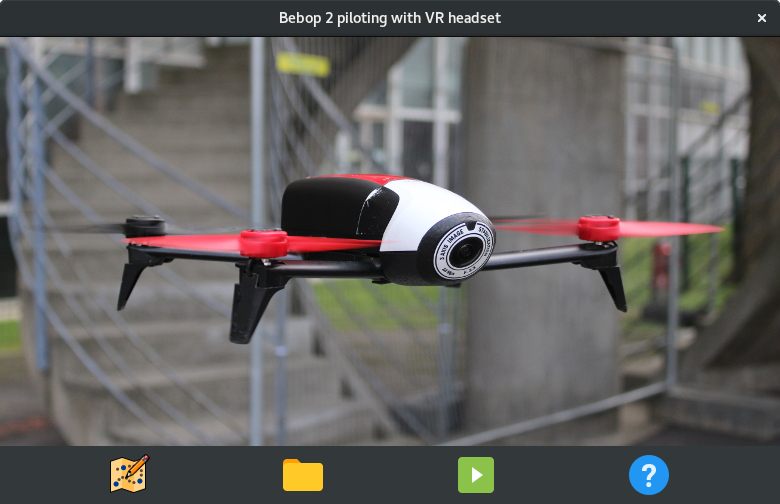
\includegraphics[scale=0.4]{main-GUI.png}
		\end{center}
	\end{frame}
	
%________________________________________________________________________________________________	


	\begin{frame}
		\begin{center}
		\frametitle{Scénario : 3 - Saisie d'un plan de vol}

        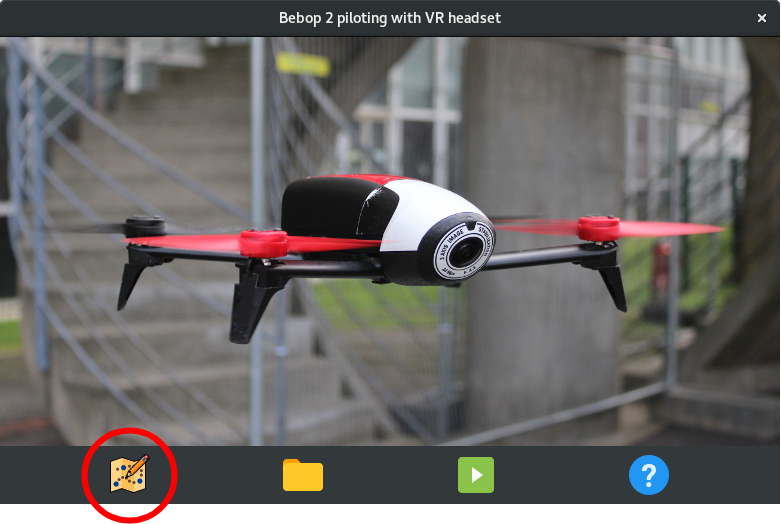
\includegraphics[scale=0.4]{createMap.png}
		\end{center}
	\end{frame}
	
%________________________________________________________________________________________________	


	\begin{frame}
		\begin{center}
		\frametitle{Scénario : 3 - Saisie d'un plan de vol}

        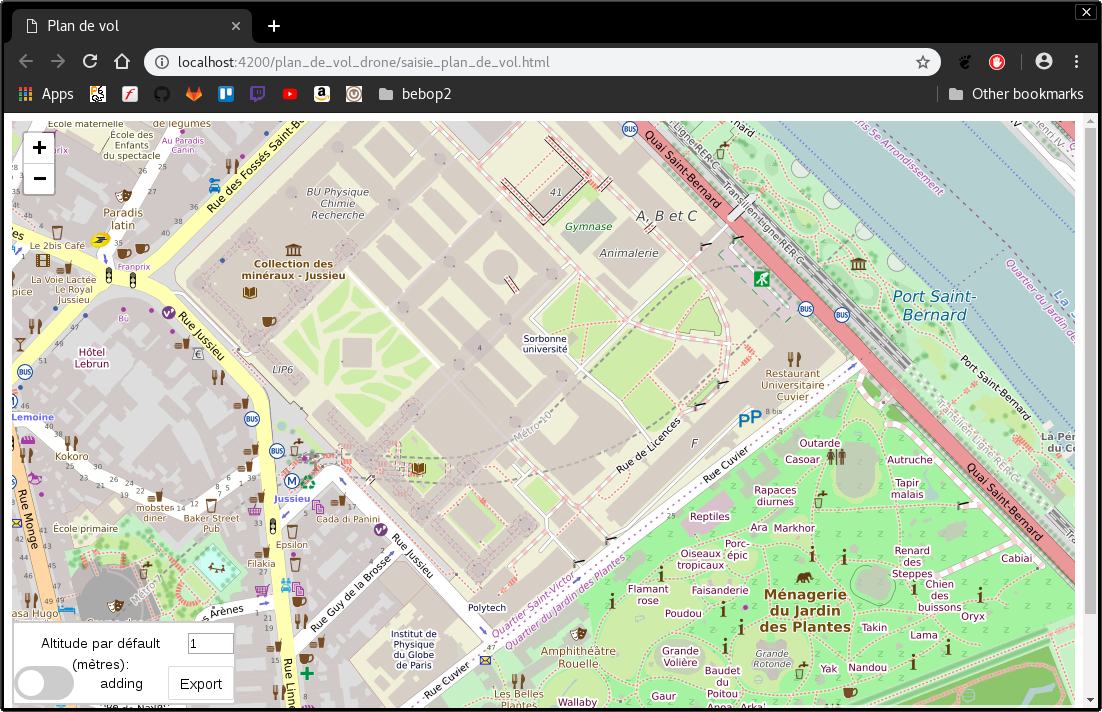
\includegraphics[scale=0.28]{map-GUI.png}
		\end{center}
	\end{frame}
	
%________________________________________________________________________________________________	


	\begin{frame}
		\begin{center}
		\frametitle{Scénario : 4 - Préparation du vol}
        \begin{enumerate}
		    \item Connexion du PC au wifi du drone
		    \item Connexion de l'iPod au réseau local et démarrage de l'application sur l'iPod
		    \item Mise en place de l'iPod dans le masque FPV
		\end{enumerate}
		
		\end{center}
	\end{frame}
	
%________________________________________________________________________________________________	


	\begin{frame}
		\begin{center}
		\frametitle{Scénario : 5 - Choix du plan de vol}

        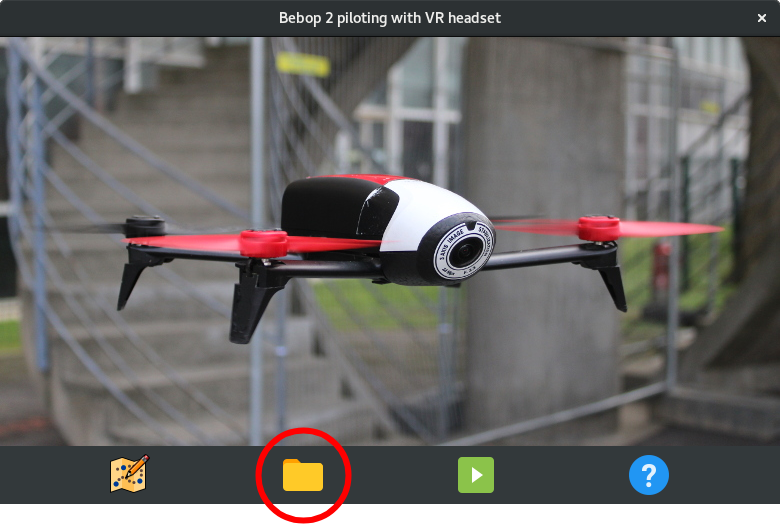
\includegraphics[scale=0.4]{chooseFile.png}
		\end{center}
	\end{frame}
	
%________________________________________________________________________________________________	


	\begin{frame}
		\begin{center}
		\frametitle{Scénario : 5 - Choix du plan de vol}

        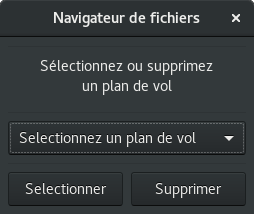
\includegraphics[scale=0.6]{selecteur-GUI.png}
		\end{center}
	\end{frame}
	
	
	
%________________________________________________________________________________________________	


	\begin{frame}
		\begin{center}
		\frametitle{Scénario : 6 - Décollage du drone}

        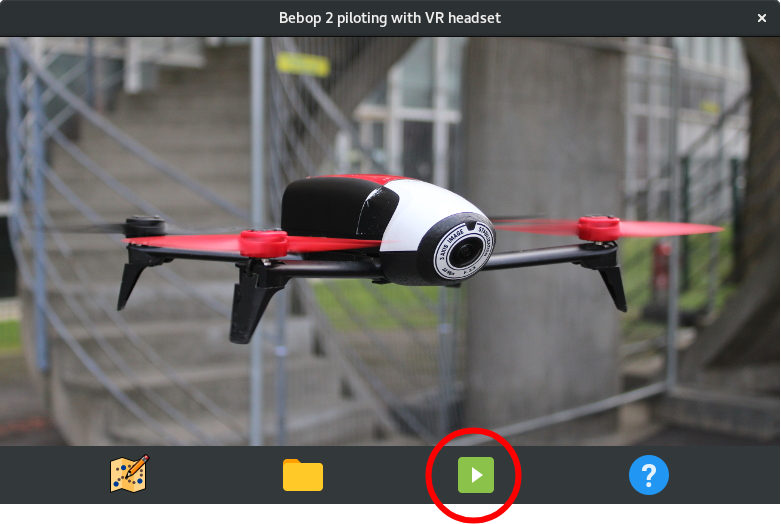
\includegraphics[scale=0.4]{startFlight.png}
		\end{center}
	\end{frame}
	
%________________________________________________________________________________________________	


	\begin{frame}
		\begin{center}
		\frametitle{Scénario : 6 - Décollage du drone}
        L'utilisateur peut enfiler le masque FPV et ensuite secouer la tête pour faire décoller le drone.\\
        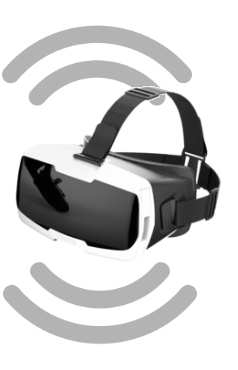
\includegraphics[scale=0.4]{shake.png}
		\end{center}
	\end{frame}
	
%________________________________________________________________________________________________	


	\begin{frame}
		\begin{center}
		\frametitle{Scénario : 7 - Fin du vol}
        L'utilisateur peut enclencher un arrêt d'urgence en secouant la tête ou bien attendre que le drone ait fini le vol et atterrisse de lui-même.\\
        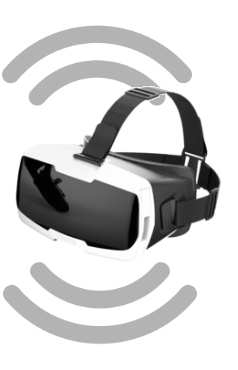
\includegraphics[scale=0.4]{shake.png}
		\end{center}
	\end{frame}
	
%________________________________________________________________________________________________	


	\begin{frame}
		\section{Architecture Matérielle}
		\begin{center}
		\frametitle{Architecture Matérielle}

       
        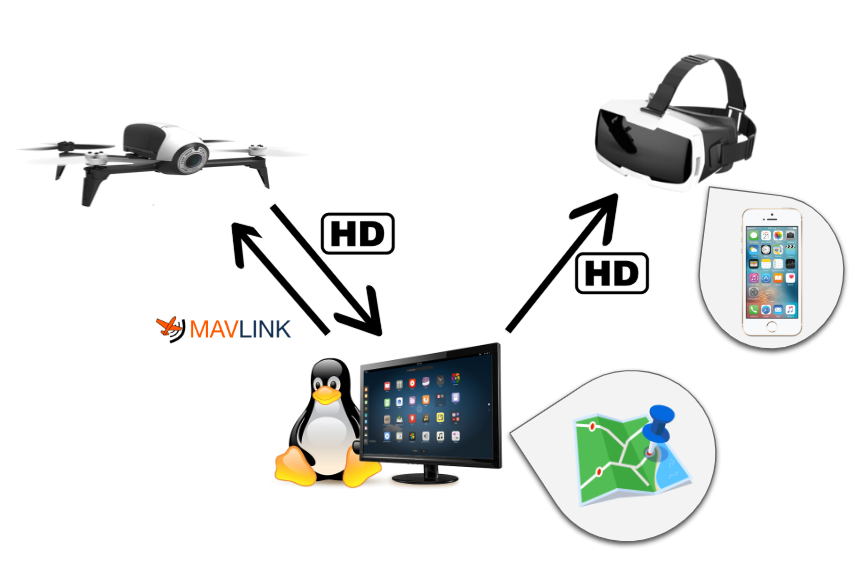
\includegraphics[scale=0.6]{archi_materielle.png}
		\end{center}
	\end{frame}
	
%________________________________________________________________________________________________	


	\begin{frame}
	\section{Architecture Logicielle}
		\begin{center}
		\frametitle{Architecture Logicielle : interface utilisateur}

       
        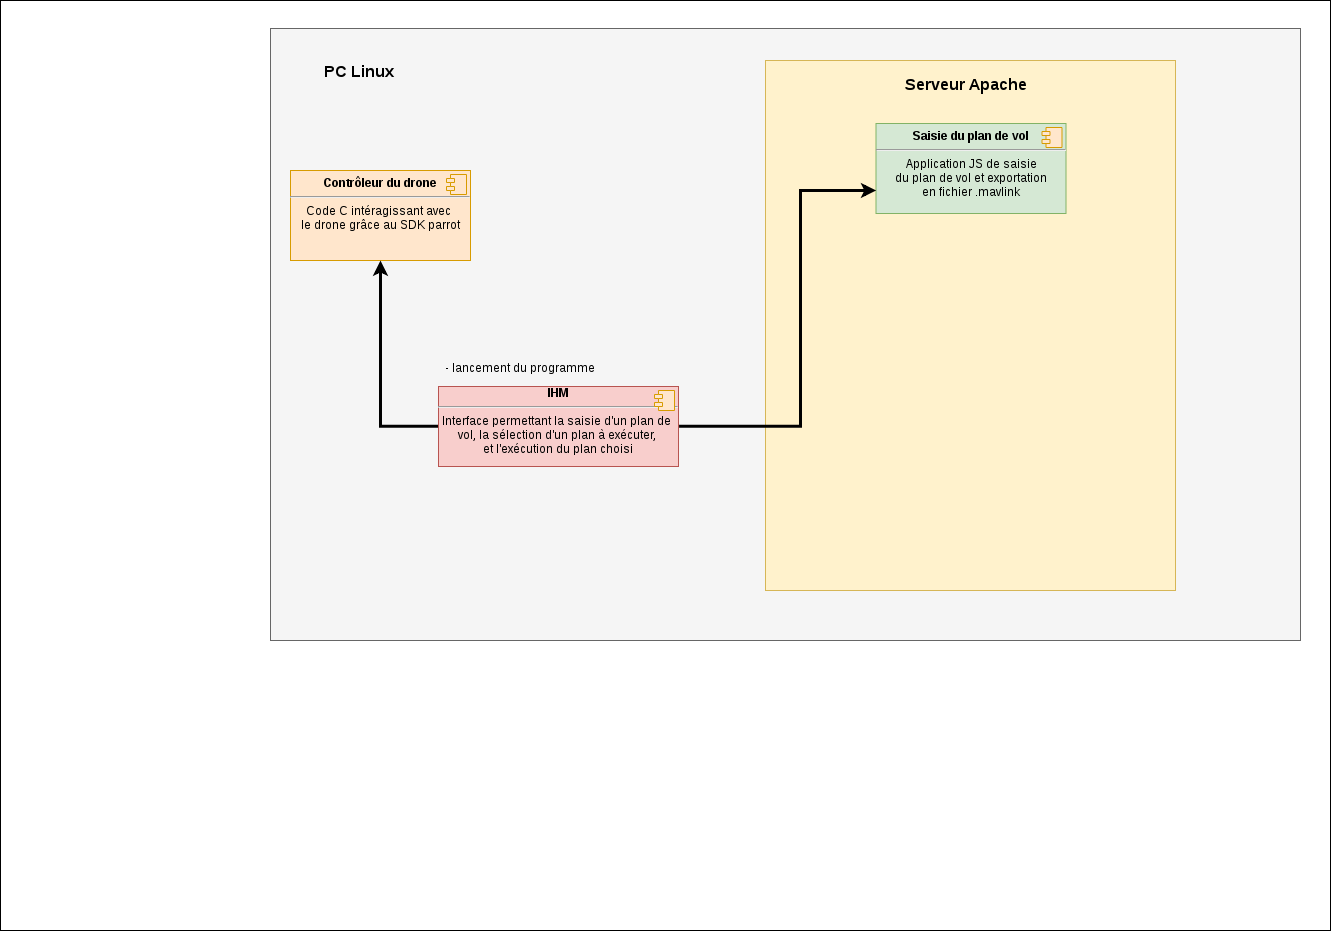
\includegraphics[scale=0.24]{01_archi_logicielle_IHM.png}
		\end{center}
	\end{frame}
	
%________________________________________________________________________________________________


	\begin{frame}
		
		\begin{center}
		\frametitle{Architecture Logicielle : controle du drone}

       
        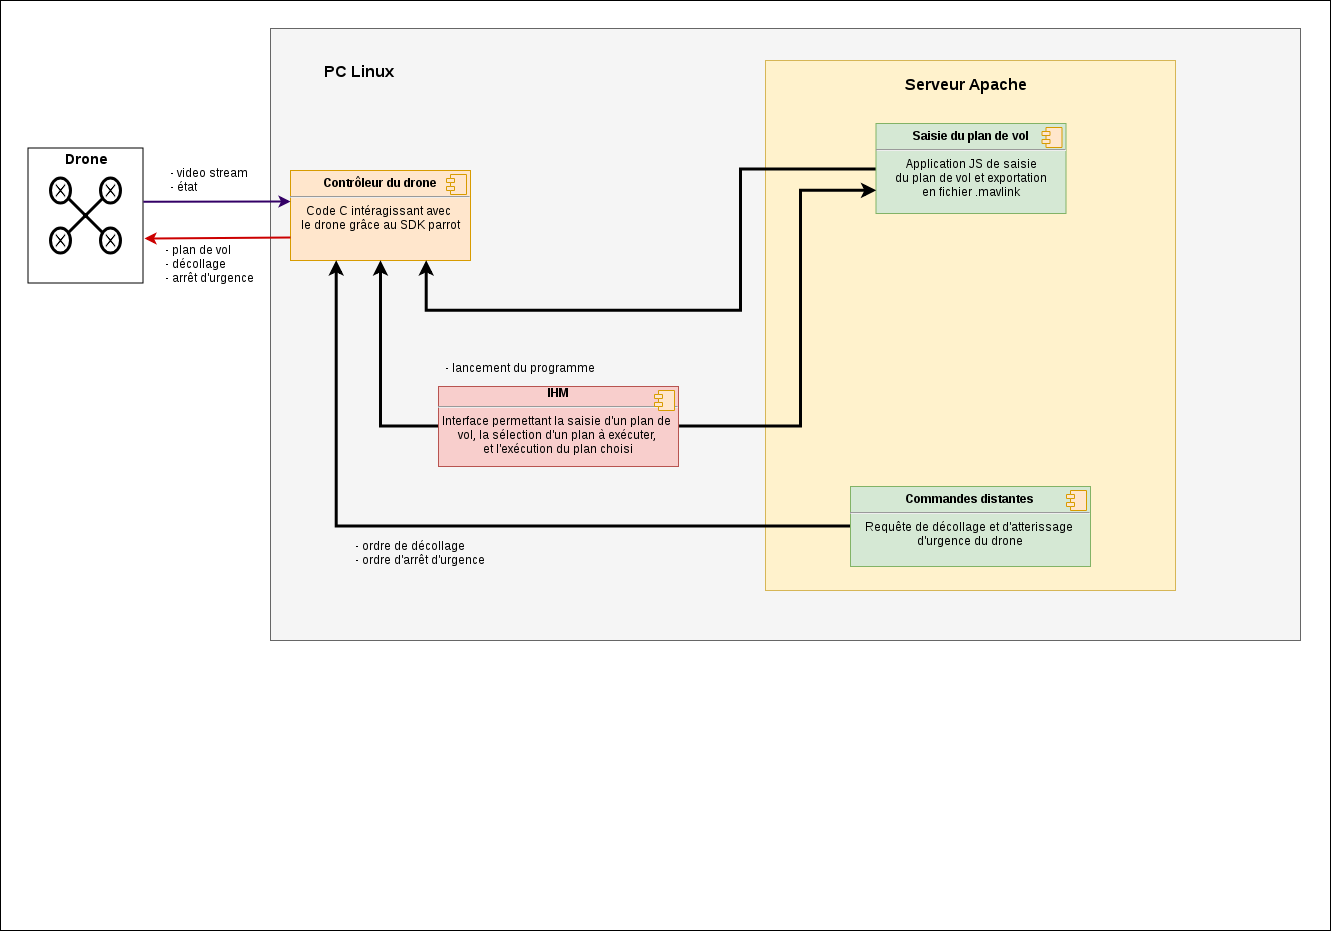
\includegraphics[scale=0.24]{02_archi_logicielle_controle_drone.png}
		\end{center}
	\end{frame}
	
	%________________________________________________________________________________________________

	\begin{frame}
		\begin{center}
		\frametitle{Architecture Logicielle : contrôle avec l'iPod}

       
        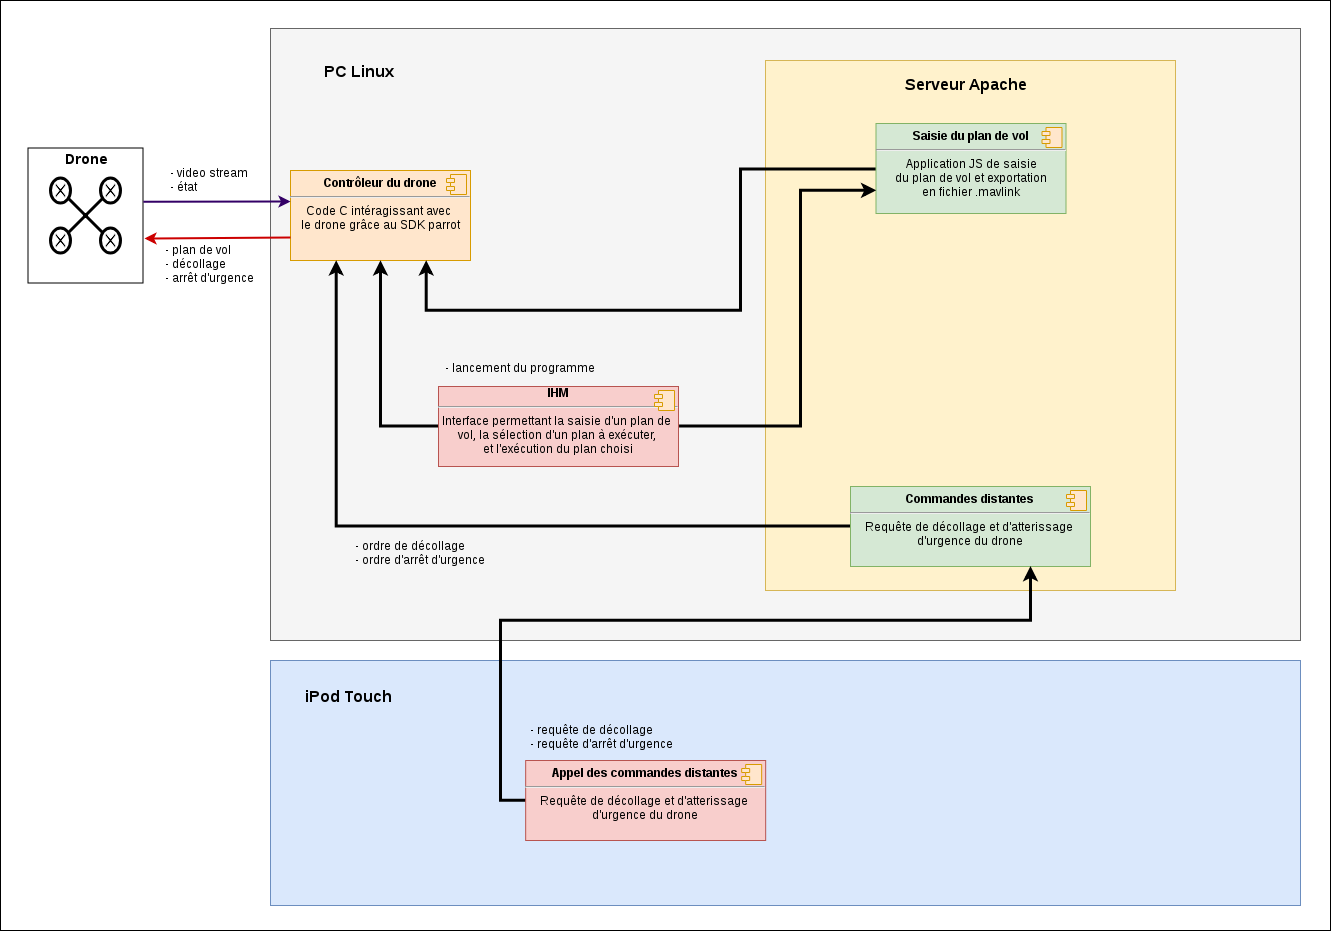
\includegraphics[scale=0.24]{03_archi_logicielle_iPod.png}
		\end{center}
	\end{frame}


%________________________________________________________________________________________________

	\begin{frame}
		\begin{center}
		\frametitle{Architecture Logicielle : retour vidéo sur l'iPod}

       
        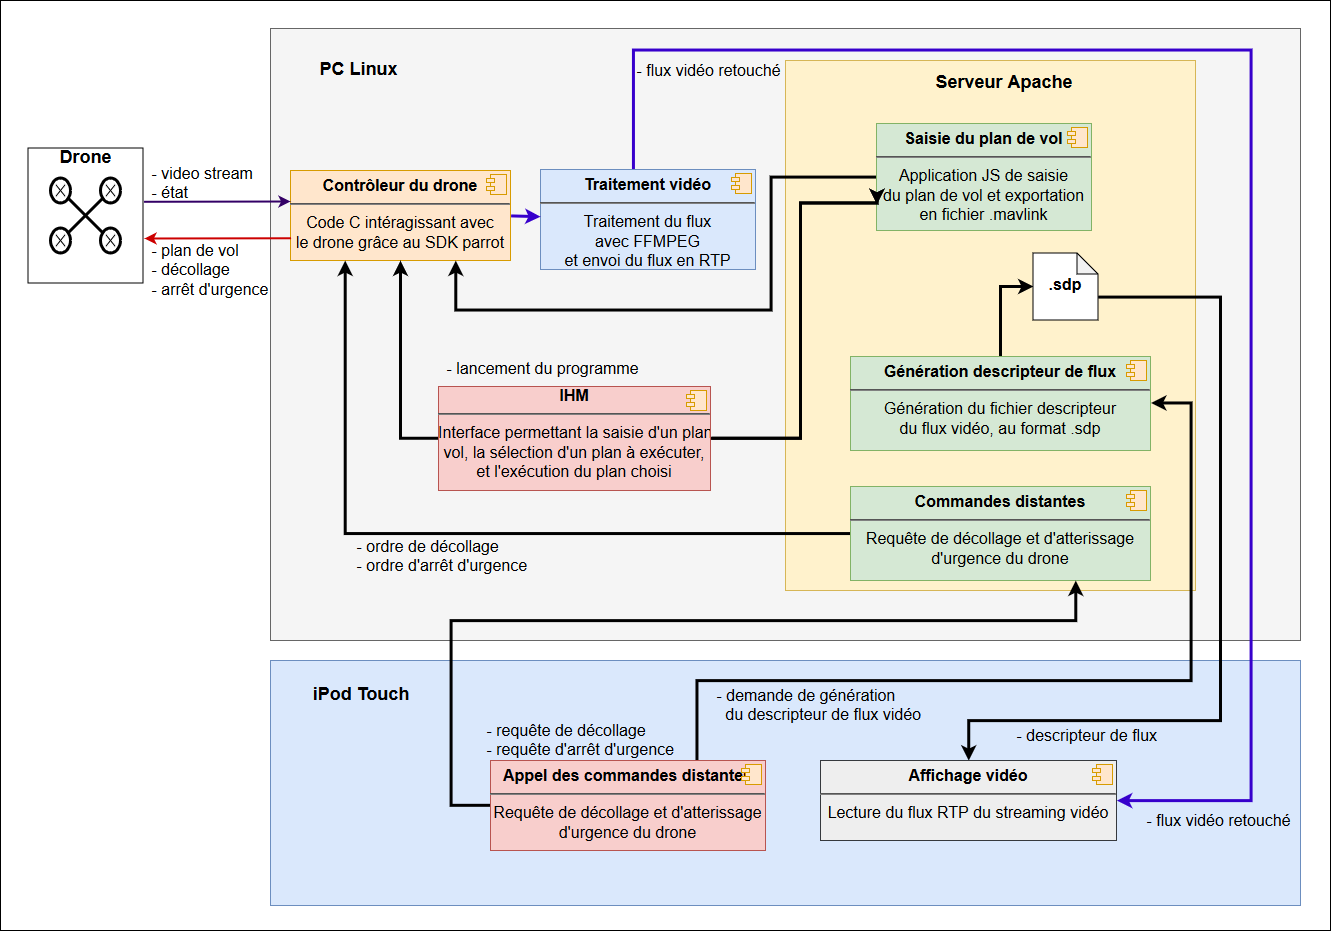
\includegraphics[scale=0.24]{04_archi_logicielle_complete.png}
		\end{center}
	\end{frame}
	
%________________________________________________________________________________________________
	
	
	\begin{frame}
		\section{Test Effectués}
		\begin{center}
		\frametitle{Tests effectués}
           	\begin{itemize}
           	    \item Saisie d'un plan de vol avec la fonctionnalité dédiée
                \item Démarrage du drone par un mouvement de tête avec le masque FPV contenant l'iPod
                \item Exécution du plan de vol choisi en totalité
                \item Arrêt d'urgence par un mouvement de tête avec le masque FPV contenant l'iPod
                \item Affichage de la vidéo du drone sur l'iPod en temps réel, avec un traitement pour la vue FPV (une image par oeil)
            \end{itemize}
		\end{center}
	\end{frame}

	
%________________________________________________________________________________________________	
	
	\begin{frame}
	\section{Déploiement}
		\begin{center}
		\frametitle{Déploiement}
		\begin{itemize}
	    \item	L'archive contient un script Makefile permettant d'extraire au bon endroit les différents composants de l'application.\\
	    \item	Les outils requis tels que GTK+ 3.0, un serveur Lamp et FFMPEG devront être installés par l'utilisateur au préalable.\\
	    \item	Le serveur devra être paramétré pour donner accès au répertoire "public".\\
		\end{itemize}
		\end{center}
	\end{frame}
	
%________________________________________________________________________________________________	
	
	\begin{frame}
		\begin{center}
		\frametitle{Déploiement : action du Makefile}
		%mettre schéma déploiement
        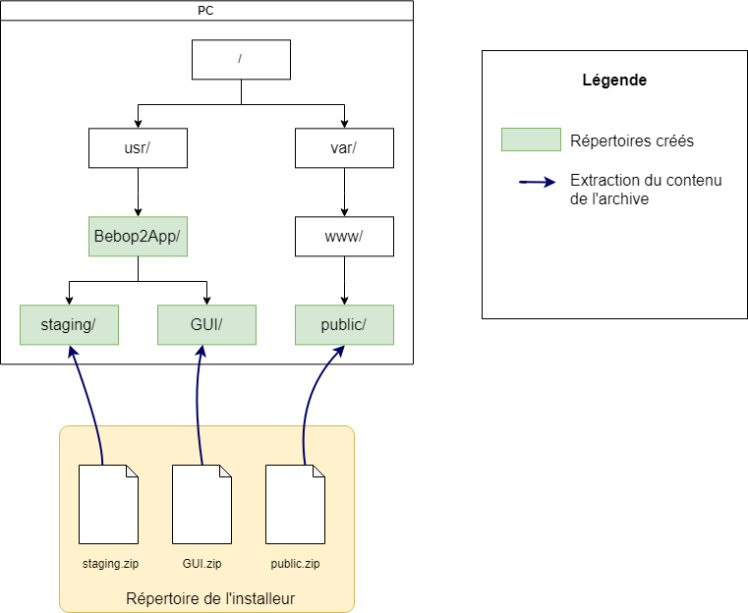
\includegraphics[scale=0.3]{deploiement.png}
		\end{center}
	\end{frame}
	
%________________________________________________________________________________________________	
	
	\begin{frame}
		\begin{center}
		\frametitle{Déploiement : contenu de l'archive}
        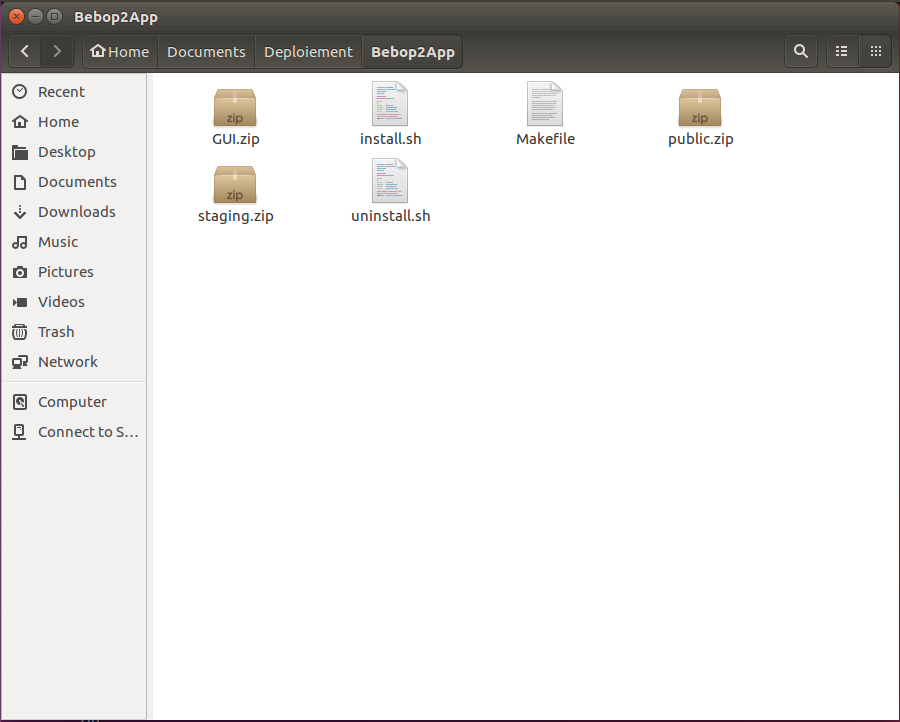
\includegraphics[scale=0.3]{result_deploiment_1.png}
		\end{center}
	\end{frame}
	
%________________________________________________________________________________________________	
	
	\begin{frame}
		\begin{center}
		\frametitle{Déploiement : exécution du Make}
        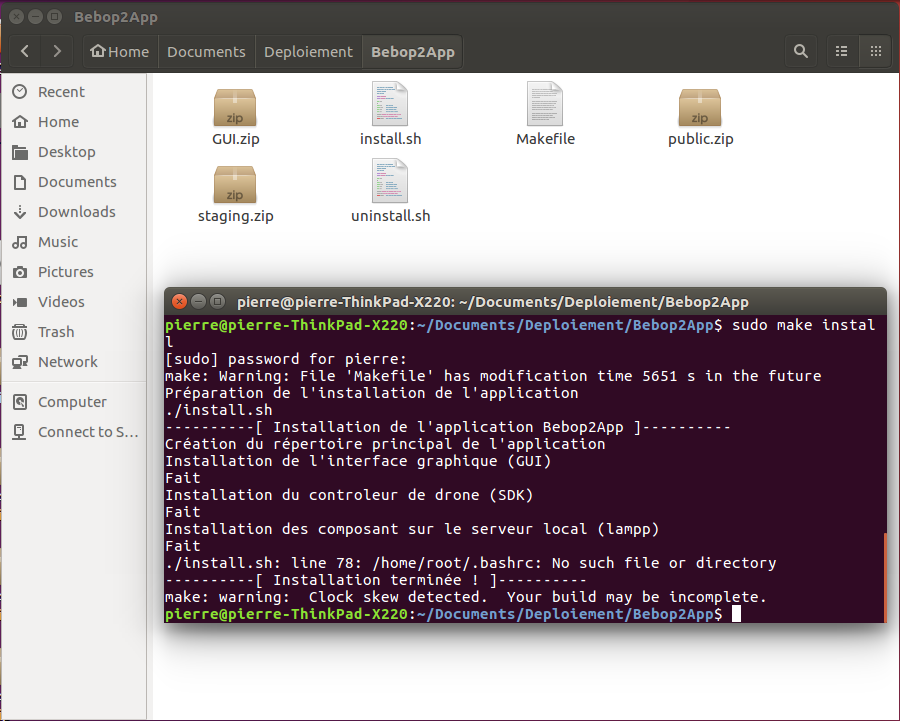
\includegraphics[scale=0.3]{result_deploiment_2.png}
		\end{center}
	\end{frame}

%________________________________________________________________________________________________	
	
	\begin{frame}
		\begin{center}
		\frametitle{Déploiement : résultat côté controle du drone et IHM}
        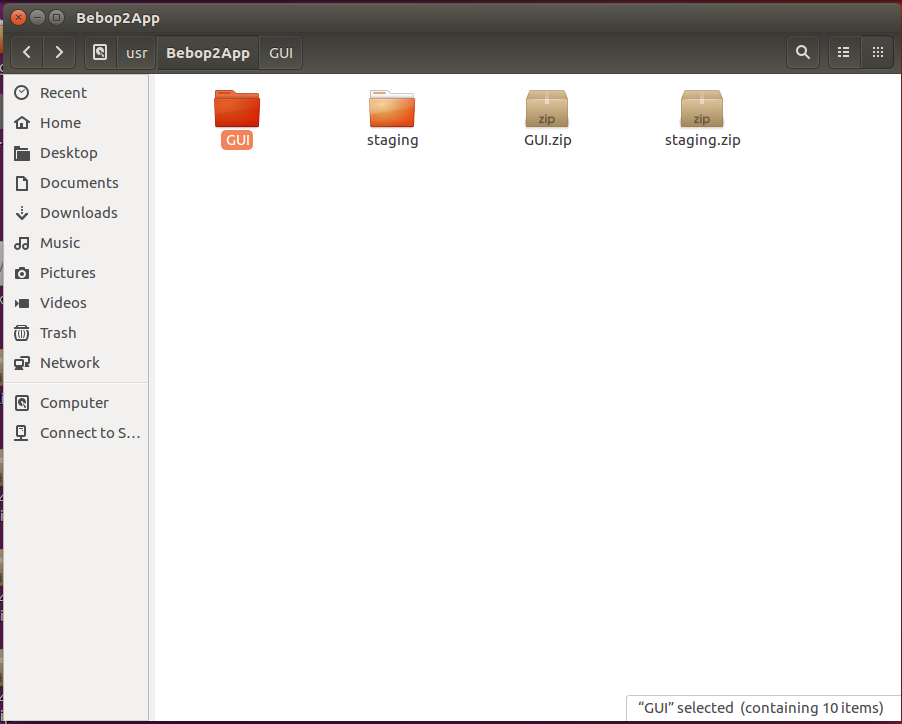
\includegraphics[scale=0.3]{result_deploiment_3.png}
		\end{center}
	\end{frame}

%________________________________________________________________________________________________	
	
	\begin{frame}
		\begin{center}
		\frametitle{Déploiement : résultat côté serveur}
        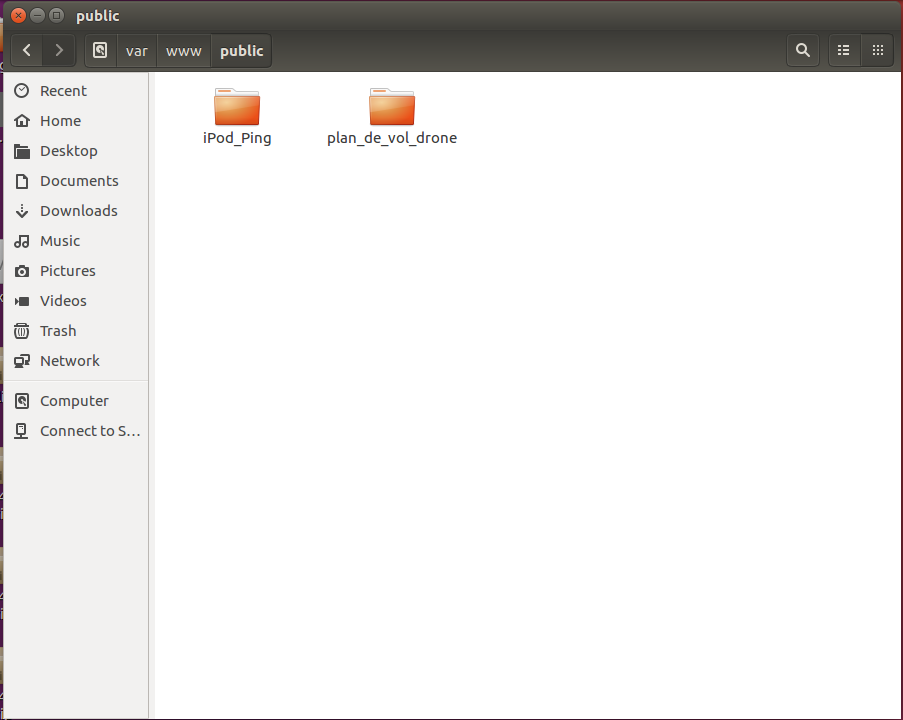
\includegraphics[scale=0.3]{result_deploiment_4.png}
		\end{center}
	\end{frame}




%________________________________________________________________________________________________	
	
	\begin{frame}
	\section{Problèmes rencontrés}
		\begin{center}
		\frametitle{Problèmes rencontrés}
        \begin{enumerate}
            \item Calibration du drone après chaque arrêt d'urgence (choc ou inclinaison trop forte du drone)
            \item Transmission du flux vidéo à l'iPod
            \item Perte du signal GPS sur campus de l'UPMC
             \end{enumerate}
		\end{center}
	\end{frame}

%________________________________________________________________________________________________	
	
	\begin{frame}
		\section{Répartition du travail}
		\begin{center}
		\frametitle{Diagramme de Gantt}
        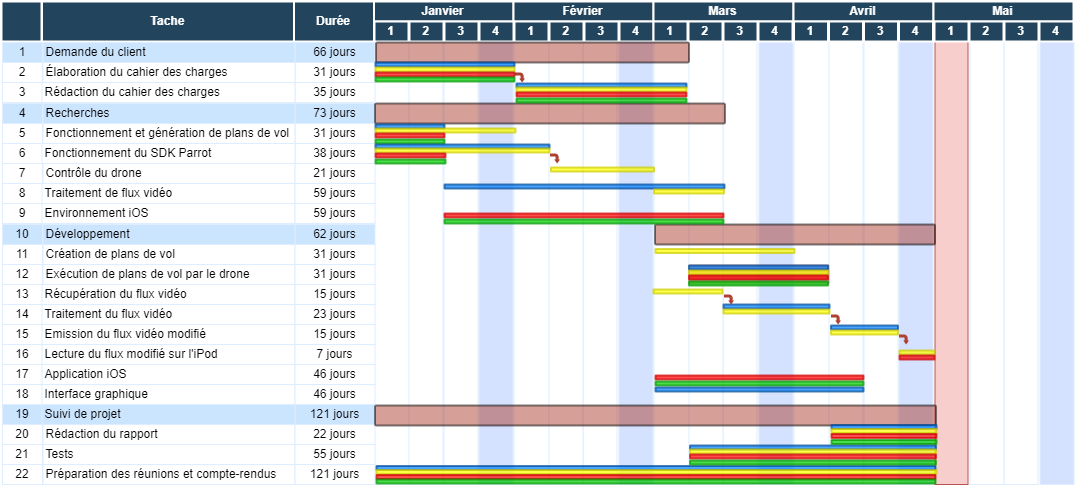
\includegraphics[scale=0.26]{gantt.png}
		\end{center}
	\end{frame}

%________________________________________________________________________________________________	
	
	\begin{frame}
		\begin{center}
		\frametitle{Répartition des tâches}
        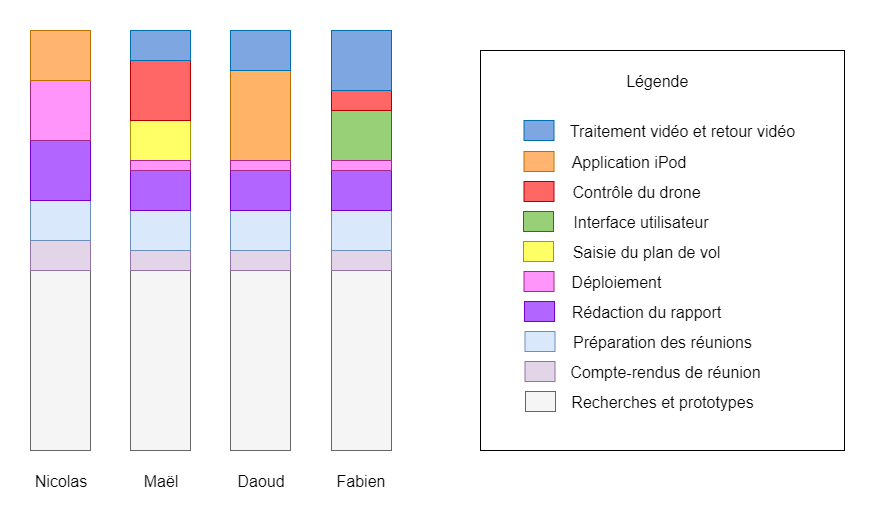
\includegraphics[scale=0.3]{repartition_taches.png}
		\end{center}
	\end{frame}

%________________________________________________________________________________________________	
	
	\begin{frame}
	    \section{Conclusion}
		\begin{center}
		\frametitle{Conclusion}
		\end{center}
	\end{frame}



%________________________________________________________________________________________________	
	
\end{document}
